\documentclass[10pt]{report}

\usepackage{enumerate} % for enumerate counter
\usepackage{subcaption} % for subfigures
\usepackage{amsthm} % for QED
\usepackage{mathtools} % for delimiter

\usepackage{listings} % for code
\lstset{ 
	language=R,
	basicstyle=\footnotesize\ttfamily,
	numbers=none,
	stepnumber=1,
	numbersep=8pt,
	showspaces=false,
	showstringspaces=false,
	showtabs=false,
	frame=single,
	tabsize=2,
	captionpos=t,
	breaklines=true,
	breakatwhitespace=false
} 

\usepackage{float} % for figure [H]
\usepackage{booktabs} % for tabular
\usepackage{caption} % for \caption*
\usepackage[export]{adjustbox} % for valign=t
\usepackage{array} % for column type m
\usepackage{verbatim}
\usepackage{graphicx}
%\graphicspath{ {imgs/} }
\usepackage{fancyhdr}
\usepackage{amssymb}
\usepackage{amsmath}

%%%%%%Pagination
\setlength{\topmargin}{-.3 in}
\setlength{\oddsidemargin}{0in}
\setlength{\evensidemargin}{0in}
\setlength{\textheight}{9.in}
\setlength{\textwidth}{6.5in}

%Cover
\newcommand{\hwTitle}{Homework \#5}
\newcommand{\hwCourse}{Applied Statistics}
\newcommand{\hmClassInstructor}{Professor Lulu Kang}

\title{
	\vspace{2in}
	\textmd{\textbf{\hwCourse\\\hwTitle}}\\
	\vspace{0.3in}\large{\textit{\hmClassInstructor}}
	\vspace{3in}
}
\author{\textbf{Zhihao Ai}}
\date{}

%Header
\pagestyle{fancy}
\fancyhead[L]{Zhihao Ai}
\fancyhead[C]{Math 484}
\fancyhead[R]{Homework 5}
%%%%%%

%Global settings
%\everymath{\displaystyle}
\setlength\parindent{0pt}

%Custom commands
\newcommand{\ds}{\displaystyle}
\newcommand{\ts}{\textstyle}

\newcolumntype{N}{>$ c <$}
\newcolumntype{M}[1]{>{\centering\arraybackslash $}m{#1}<{$}}

\newcommand{\abs}[1] {\left| #1 \right|}

\DeclarePairedDelimiter\autoparen{(}{)}
\newcommand{\pa}[1]{\autoparen*{#1}}

\newcommand{\var} {\text{var}}

\newcommand{\m}[1] {\mathbf{#1}}

\begin{document}

\maketitle

\section*{Problem 1}
(Ex. 9.13) \textbf{Lung pressure}
\begin{enumerate}[a.]
	\item 
	Prepare separate dot plots for each of the three predictor variables. Are there any noteworthy features in these plots? Comment.
	\begin{figure}[H]
		\centering
		\begin{subfigure}[b]{.3\linewidth}
			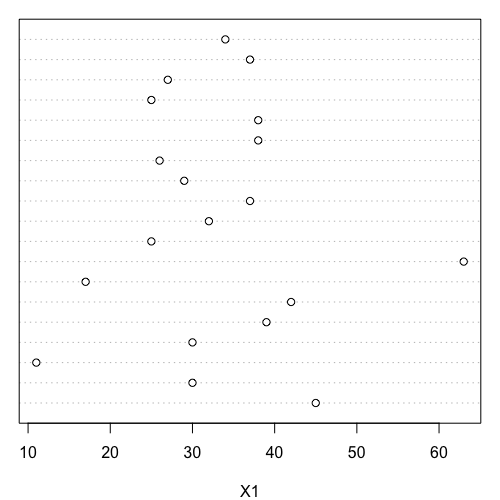
\includegraphics[width=\linewidth]{p1/13a_x1.png}
		\end{subfigure}
		\begin{subfigure}[b]{.3\linewidth}
			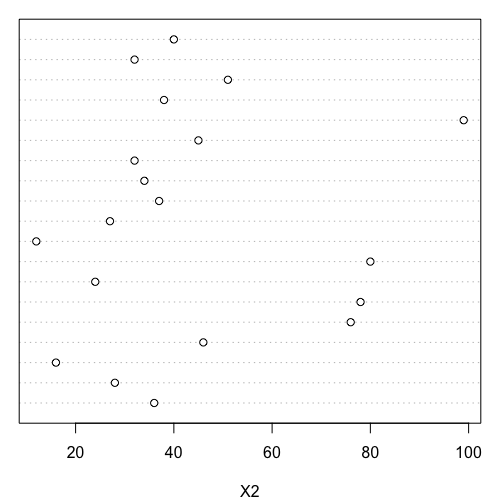
\includegraphics[width=\linewidth]{p1/13a_x2.png} 
		\end{subfigure}
		\begin{subfigure}[b]{.3\linewidth}
			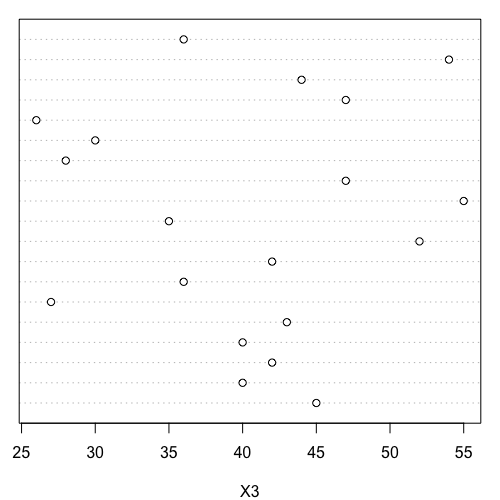
\includegraphics[width=\linewidth]{p1/13a_x3.png} 
		\end{subfigure}
	\end{figure}
	Both $X_1$ and $X_2$ are relatively concentrated in the lower part of each range, whereas $X_3$ is randomly scattered in its range. There are several outliers in dot plots of $X_1$ and $X_2$.
	
	\item 
	Obtain the scatter plot matrix. Also obtain the correlation matrix of the $X$ variables. What do the scatter plots suggest about the nature of the functional relationship between $Y$ and each of the predictor variables? Are any serious multicollinearity problems evident? Explain.
	
	Scatter plot matrix:
	\begin{figure}[H]
		\centering
		\vspace{-4ex}
		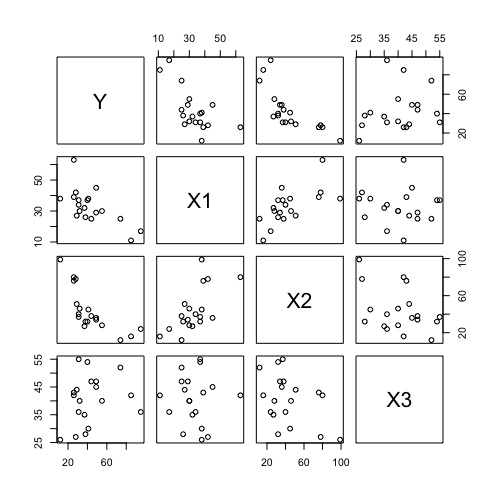
\includegraphics[width=.5\linewidth]{p1/13b.png}
		\vspace{-5ex}
	\end{figure}
	Correlation matrix:
	\lstinputlisting{p1/13b.txt}
	The scatter plots suggest that there exists negative correlation between $Y$ and both $X_1$ and $X_2$, and no clear correlation between $Y$ and $X_3$ is shown. The correlation coefficient between $X_1$ and $X_2$ is 0.65, indicating a moderate correlation between them, which could results in muticollinearity problems.
	
	\item 
	Fit the multiple regression function containing the three predictor variables as first-order terms. Does it appear that all predictor variables should be retained?
	\lstinputlisting{p1/13c.txt}
	The $p$-values of $\hat{\beta_1}$ and $\hat{\beta_3}$ are not significant, so it appears not all predictor variables should be retained.
\end{enumerate}

\section*{Problem 2}
(Ex. 9.14) Refer to \textbf{Lung pressure} Problem 9.13
\begin{enumerate}[a.]
	\item 
	Using first-order and second-order terms for each of the three predictor variables (centered around the mean) in the pool of potential $X$ variables (including cross products of the first-order terms), find the three best hierarchical subset regression models according to the $R_{a,p}^2$ criterion.
	\begin{figure}[H]
		\centering
		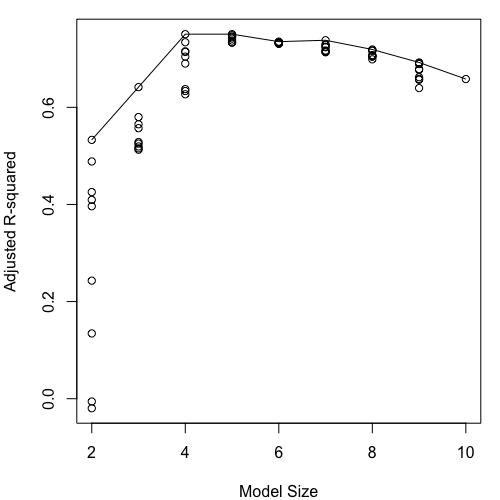
\includegraphics[width=.5\linewidth]{p2/14a.png}
	\end{figure}
	The three best subsets are
	\lstinputlisting{p2/14a.txt}
	The $R_{a,p}^2$'s of the models containing $\{X_1, X_2, X_1^2, X_2^2\}$, $\{X_1, X_2, X_1 X_2\}$ and $\{X_1, X_3, X_1^2, X_2 X_3\}$ are 0.7506701, 0.7506631 and 0.7485086, correspondingly.
	
	\item 
	Is there much difference in $R_{a,p}^2$ for the three best subset models?
	
	There is little difference between them.
\end{enumerate}

\section*{Problem 3}
(Ex. 10.13) \textbf{Cosmetics sales}
\begin{enumerate}[a.]
	\item 
	State the regression model to be employed and fit it to the data.
	
	First order multiple regression model is to be employed.
	\lstinputlisting{p3/13a.txt}
	Fitting the model to the data, we have $\hat{Y}=1.0233 + 0.9657 x_1 + 0.6292 x_2 + 0.6760 x_3$.
	
	\item 
	Test whether there is a regression relation between sales and the three predictor variables; use $\alpha = .05$. State the alternatives, decision rule, and conclusion.
	
	The alternatives are
	\begin{align*}
		H_0 &: \beta_1 = \beta_2 = \beta_3 = 0\\
		H_a &: \text{not all } \beta_i=0, i=1,2,3
	\end{align*}
	The test statistic is
	\[
	F^* = \frac{MSR}{MSE}
	\]
	The decision rule is
	\begin{align*}
		\text{If } F^* \le F(1-\alpha; p-1, n-p) = 2.838745, \text{ conclude } H_0\\
		\text{If } F^* > F(1-\alpha; p-1, n-p) = 2.838745, \text{ conclude } H_a
	\end{align*}
	The ANOVA table is shown below:
	\lstinputlisting{p3/13b.txt}
	So, the test statistic $F^* = 38.28 > 2.838745$, we conclude $H_a$, that not all $\beta_i$ is zero.
	
	\item 
	Test for each of the regression coefficients $\beta_k (k=1,2,3)$ individually whether or not $\beta_k=0$; use $\alpha = .05$ each time. Do the conclusions of these tests correspond to that obtained in part (b)?
	
	The alternatives are
	\begin{align*}
		H_0 &: \beta_k = 0\\
		H_a &: \beta_k \ne 0
	\end{align*}
	The test statistic is
	\[
	t^* = \frac{\hat{\beta}_k}{s\{\hat{\beta}_k\}}
	\]
	The decision rule is
	\begin{align*}
		\text{If } \abs{t^*} \le t(1-\alpha/2; n-p) = 2.021075, \text{ conclude } H_0\\
		\text{If } \abs{t^*} > t(1-\alpha/2; n-p) = 2.021075, \text{ conclude } H_a
	\end{align*}
	\lstinputlisting{p3/13c.txt}
	According to the table above, $t^*$ for each $\beta_k$ is smaller than 2.021075. Therefore, for each $\beta_k$, we conclude $H_0$. It doesn't correspond to the conclusion obtain in part (b).
	
	\item 
	Obtain the correlation matrix of the $X$ variables.
	\lstinputlisting{p3/13d.txt}
	
	\item 
	What do the results in parts (b), (c), and (d) suggest about the suitability of the data for the research objective?
	
	The results suggest that there exists serious multicollinearity in the data, so it's not suitable for the research objective.
\end{enumerate}

\section*{Problem 4}
(Ex. 10.20) Refer to \textbf{Lung pressure} Problem 9.13 and 9.14. The subset regression model containing first-order terms for $X_1$ and $X_2$ and the cross-product term $X_1 X_2$ is to be evaluated in detail.
\begin{enumerate}[a.]
	\item 
	Obtain the residuals and plot them separately against $\hat{Y}$ and each of the three predictor variables. On the basis of these plots, should any further modifications of the regression model be attempted?
	\begin{figure}[H]
		\centering
		\begin{subfigure}[b]{.25\linewidth}
			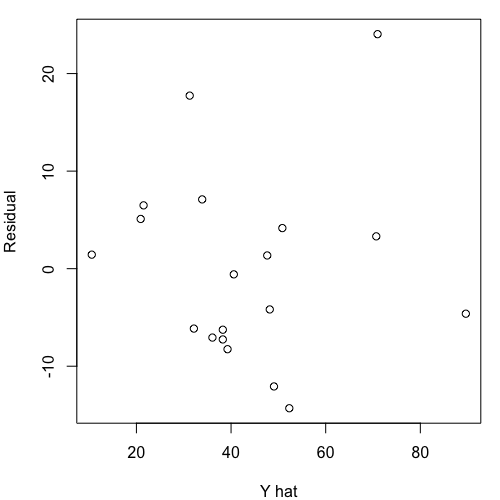
\includegraphics[width=\linewidth]{p4/20a_yhat.png}
		\end{subfigure}%%
		\begin{subfigure}[b]{.25\linewidth}
			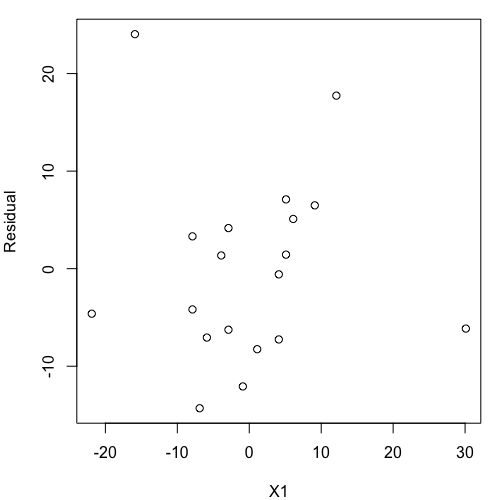
\includegraphics[width=\linewidth]{p4/20a_x1.png} 
		\end{subfigure}%%
		\begin{subfigure}[b]{.25\linewidth}
			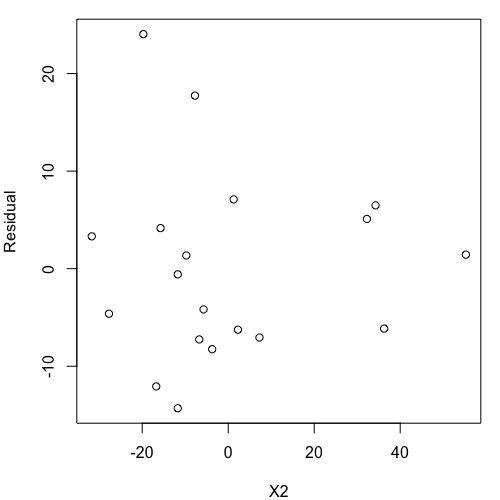
\includegraphics[width=\linewidth]{p4/20a_x2.png} 
		\end{subfigure}%%
		\begin{subfigure}[b]{.25\linewidth}
			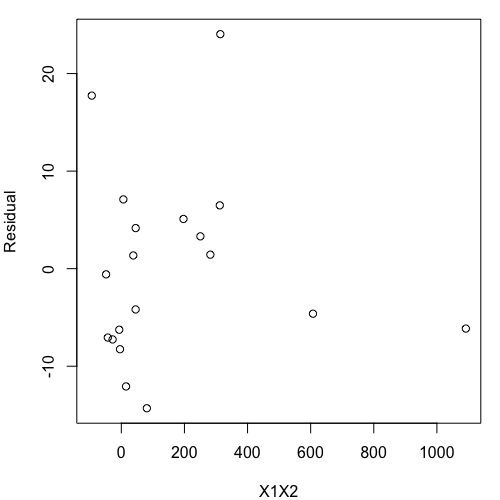
\includegraphics[width=\linewidth]{p4/20a_x1x2.png} 
		\end{subfigure}
	\end{figure}
	The residual variance may not be constant as shown in the plots above. Transformation on some of the variables is necessary. Also, there seem to be outliers in the data.
	
	\item 
	Prepare a normal probability plot of the residuals. Also obtain the coefficient of correlation between the ordered residuals and their expected values under normality. Does the normality assumption appear to be reasonable here?
	\begin{figure}[H]
		\centering
		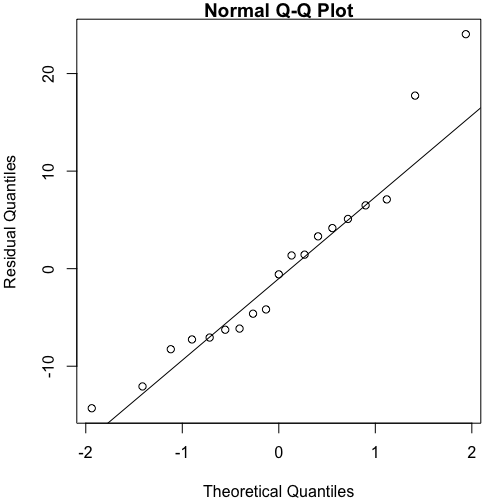
\includegraphics[width=.4\linewidth]{p4/20b.png}
	\end{figure}
	The normal quantiles are calculated as
	\[
	z_i = \Phi^{-1} \pa{\frac{i-0.375}{n+0.25}}
	\]
	where $\Phi^{-1}(\cdot)$ is the inverse CDF of standard normal distribution. Then with the ordered residuals, we obtain 0.9633751 as the coefficient of correlation between them. Using table B.6, the critical value when $n=19$ using a 0.01 significance level is about 0.923. Since $0.9633751 > 0.923$, the normality assumption appear to be reasonable.
	
	\item 
	Obtain the variance inflation factors. Are there any indications that serious multicollinearity problems are present? Explain.
	
	Calling \verb|vif| on the model, we have
	\lstinputlisting{p4/20c.txt}
	Since $\max{VIF} = 22.47 > 10$, multicollinearity problems exist.
	
	\item 
	Obtain the studentized deleted residuals and identify any outlying $Y$ observations. Use the Bonferroni outlier test procedure with $\alpha = .05$. State the decision rule and conclusion.
	
	The alternatives are
	\begin{align*}
	H_0 &: \text{$Y_i$ is not an outlier}\\
	H_a &: \text{$Y_i$ is an outlier}
	\end{align*}
	Studentized deleted residual is given by
	\[
	t_i = e_i \pa{\frac{n-p-1}{SSE(1-h_{ii})-e_i^2}}^{1/2}
	\]
	The decision rule is
	\begin{align*}
	\text{If } \abs{t_i} \le t(1-\alpha/2n; n-p-1) = 3.64871, \text{ conclude } H_0\\
	\text{If } \abs{t_i} > t(1-\alpha/2n; n-p-1) = 3.64871, \text{ conclude } H_a
	\end{align*}
	The $t_i$'s are %rstudent()
	\lstinputlisting{p4/20d.txt}
	The absolute values of the $t_i$'s are all smaller than 3.64871. Therefore, we conclude $H_0$, that there is no outlying $Y$ observation at the $\alpha=0.05$ level. However, $t_7$, the largest residual among them, is close to 3.64871, and actually it would be identified as outlier with respect to $Y$ if $\alpha = .1$.
	
	\item 
	Obtain the diagonal elements of the hat matrix. Using the rule of thumb in the text, identify any outlying $X$ observations. Are your findings consistent with those in Problem 9.13a? Should they be? Discuss.
	
	The diagonal elements of $H$ are %hatvalues()
	\lstinputlisting{p4/20e.txt}
	If $h_{ii}$ is larger than $2p/n = 0.4210526$, the corresponding observation is outlying in terms of $X$ values. Therefore, cases 3, 8, and 15 are outlying $X$ observations. The findings are consistent with those in Problem 9.13a and they should be. Because from the dot plots, we can see cases 3 and 8 are outlying in terms of $X_1$ and case 15 is outlying in terms of $X_2$.
	
	\item 
	Cases 3, 8, and 15 are moderately far outlying with respect to their $X$ values, and case 7 is relatively far outlying with respect to its $Y$ value. Obtain $DFFITS$, $DFBETAS$, and Cook's distance values for these cases to assess their influence. What do you conclude?
	
	The $DFFITS$ values of these cases are %dffits()
	\lstinputlisting{p4/20f_dffits.txt}
	According to the guideline for small to medium sized data set, $\abs{DFFITS_7}$ exceeds 1 but is close enough to 1 so the case may not be influential enough; $\abs{DFFITS_8}$ indicates that case 8 may be influential enough to require remedial action.
	
	The $DFBETAS$ values of these cases are %dfbetas()
	\lstinputlisting{p4/20f_dfbetas.txt}
	As shown above, case 7 exceeds the guideline of 1 for small to medium sized data set for $\hat{\beta}_1$, but not by too much, indicating it's potentially influential but not influential enough to require remedial action. Case 8 exceeds 1 for each estimated coefficient so remedial action is clearly required.
	
	The Cook's distance values for these cases are %cooks.distance()
	\lstinputlisting{p4/20f_cook.txt}
	The percentile values of the corresponding $D_i$ from the $F(4, 15)$ distribution are %pf()
	\lstinputlisting{p4/20f_cookpf.txt}
	$D_8$ is the 99th($\gg$50th) percentile of the distribution so case 8 has a major influence on the regression fit.
\end{enumerate}

\end{document}

